\documentclass{article}

\usepackage{arxiv}

\usepackage[utf8]{inputenc} % allow utf-8 input
\usepackage[T1]{fontenc}    % use 8-bit T1 fonts
\usepackage{hyperref}       % hyperlinks
\usepackage{url}            % simple URL typesetting
\usepackage{booktabs}       % professional-quality tables
\usepackage{amsfonts}       % blackboard math symbols
\usepackage{nicefrac}       % compact symbols for 1/2, etc.
\usepackage{microtype}      % microtypography
\usepackage{lipsum}		% Can be removed after putting your text content
\usepackage{graphicx}
\usepackage{natbib}
\usepackage{doi}
\usepackage{mathtools}
\DeclarePairedDelimiter\ceil{\lceil}{\rceil}
\DeclarePairedDelimiter\floor{\lfloor}{\rfloor}

\usepackage[english,bulgarian,ukrainian,russian]{babel}



\title{Optimal data splitting in distributed optimization \\for machine learning}

%\date{September 9, 1985}	% Here you can change the date presented in the paper title
%\date{} 					% Or removing it

\author{Gleb Molodtsov
% $ \thanks{Use footnote for providing further
%		information about author (webpage, alternative
%		address)} 
    \\
	Department of Informatics and Applied Maths \\
	Moscow Institute of Physics and Technology\\
	Moscow, Russia\\
	\texttt{molodtsov.gl@phystech.edu} \\
	%% examples of more authors
	\And
	Daniil Medyakov \\
	Department of Informatics and Applied Maths \\
	Moscow Institute of Physics and Technology\\
	Moscow, Russia \\
	\texttt{mediakov.do@phystech.edu} \\
	%% \AND
	%% Coauthor \\
	%% Affiliation \\
	%% Address \\
	%% \texttt{email} \\
	%% \And
	%% Coauthor \\
	%% Affiliation \\
	%% Address \\
	%% \texttt{email} \\
	%% \And
	%% Coauthor \\
	%% Affiliation \\
	%% Address \\
	%% \texttt{email} \\
}

% Uncomment to remove the date
%\date{}

% Uncomment to override  the `A preprint' in the header
\renewcommand{\headeright}{Technical Report}
\renewcommand{\undertitle}{Technical Report}
%\renewcommand{\shorttitle}{\textit{arXiv} Template}

%%% Add PDF metadata to help others organize their library
%%% Once the PDF is generated, you can check the metadata with
%%% $ pdfinfo template.pdf

\begin{document}
\maketitle




% keywords can be removed
% \keywords{First keyword \and Second keyword \and More}
\begin{abstract}
В данной статье рассматривается задача распределения данных по различным устройствам с учетом их производительностей. Цель настоящей работы --- получить наиболее выгодное соотношение для распределяемых данных на сервер и локальные машины. Для решения данной задачи используется оптимальный алгоритм градиентного скольжение и его применение к распределенной оптимизации при сходстве. Производится сравнение времён работы системы при равномерном и полученном оптимальном распределениях. Более высокие теоретические показатели наших решений подтверждены экспериментально.
\end{abstract}

\section{Вступление}

\subsection{Distributed optimization}
Мы рассматриваем задачу централизованной распределенной оптимизации сети, состоящей из  $m$ агентов:
Где
\subsection{Contributions}


Рассмотрим особенности постановки уравнения (2) в \cite{kovalev2022optimal}. Рассматривается сеть из $m$ агентов, которая образует звездную топологию. Первый агент является главным узлом, остальные - соединены исключительно с ним и необходимы для дополнительных вычислительных мощностей. Исследуем задачу, в которой нам требуется минимизировать среднюю лосс-функцию над некоторыми данными, и мы хотим распределить решение задачи по объектам нашей сети, вычисления в которой проводятся с помощью крайних узлов звездной топологии, а копии всех оптимизационных переменных и связь между ячейками проводится через главный (центральный) узел. Для каждой единицы сети считается функция потерь, которая измеряет разницу между вектором параметра и вектором образца. Таким образом, данная задача свелась к минимизации следующей функции: \\
\begin{equation}
    \label{eq:1}
    r(x) = \frac{1}{n} \sum \limits_{i = 1}^{n} f _i(x)
\end{equation}
Плюсы и минусы постановки:\\
Плюс постановки \ref{eq:1} заключается в том, что, применив алгоритм градиентного скольжения, мы можем со сложностью $\mathcal{O}(\sqrt{\frac{L}{\mu}})$ решить нашу минимизационную задачу для $L$-гладкой и $\mu$-сильно-выпуклой функции $r$. При этом, данная верхняя оценка содержит в себе сумму оценок локальных вычислений на крайних узлах и их коммуникаций с главным узлом. Для некоторого класса задач (где k не является большим числом) данный метод приемлем. Минус заключается в том, что при очень большом значении k алгоритм неэффективен. Такое случается, например, при высокой стоимости коммуникаций. \\
Решение проблемы \ref{eq:1}\\
Проблему \ref{eq:1} можно решить следующим образом: преобразуем функцию $r$ к следующему виду:\\
\begin{equation}
    \label{eq:2}
    r(x) = f_1(x) + \frac{1}{n}\sum\limits_{i = 1}^{n}[f_i(x) - f_1(x)]
\end{equation}
Для любого i-го выполняется следующее: $f_i$ - выпуклая функция как функция потерь локальных вычислений на вспомогательном узле, а $f_i - f_1$ не является выпуклой, однако содержит в себе коммуникационные затраты (???). Таким образом, перед нами встала задача минимизации $L$-гладкой $\mu$-сильно-выпуклой фукнций $r$ как суммы выпуклой и невыпуклой фукнций. \\
Для данной задачи была предложена модификация алгоритма градиентного скольжения \cite{kovalev2022optimal}, которая пропускает время от времени вычисление градиента одной функции. Все существующие алгоритмы градиентного скольжения были неприменимы к поставленной задаче, поскольку требовали выпуклость обеих функций и не давали оптимальных верхних оценок сложности для одновременно локального вычисления градиента и коммуникационных затрат. Однако данная модификация этого алгоритма заполняется указанные пробелы.

\section{Постановка задачи}

Рассмотрим алгоритм ускоренного экстраградиента (алгоритм 1 из \cite{kovalev2022optimal}). Рассчитаем сколько действий этот алгоритм выполняет за одну итерацию. В строчке 5 происходит 1 коммуникация, 1 локальное вычисление, 1 вычисление центрального узла и дополнительные вычисления центрального узла. В строчке 6 - 1 коммуникация, 1 локальное вычисление и 1 вычисление центрального узла. Сделаем следующие обозначения: $\tau_i$ - время одного 1 локального вычисления на i-ом устройстве, $K$ - количество итераций, $\tau_{comm}$ - время на 1 коммуникацию, $k_{some}$ - дополнительные вычисления центрального узла, $n$ - количество узлов в сети. Тогда мы можем записать общее время работы алгоритма, как:
\begin{equation}
    \label{eq:3}
    T_{sum} = 2\cdot\max(\tau_1, \tau_2, ..., \tau_n)\cdot K + 2\cdot K\cdot\tau_{comm} + \tau_1\cdot k_{some}
\end{equation}
Наша задача состоит в минимизации времени $T_{sum}$. Представим время $\tau_i$, как $\tau_i = \tau_i^{loc}\cdot b_i$, где $\tau_i^{loc}$ - время, которое тратит i-ое устройство на обработку единицы информации, поданной ему на вход, а $b_i$ - размер датасета, поданный на вход i-му устройству. $b_i$ должны удовлетворять следующим ограничениям: $\sum\limits_{i = 1}^{n} b_i = N$, где $N$ - размер всего датасета, $\delta = \frac{L}{\sqrt{b_i}}$ (данная оценка дана в \cite{kovalev2022optimal}).
Мы получили следующую задачу оптимизации:
\begin{equation}
    \label{eq:4}
    min_{\sum\limits_{i = 1}^{n} b_i = N; \delta = \frac{L}{\sqrt{b_i}}}[ 2\cdot\max(\tau_1^{loc}\cdot b_1, \tau_2^{loc}\cdot b_2, ..., \tau_n^{loc}\cdot b_n)\cdot K + 2\cdot K\cdot\tau_{comm} + \tau_1\cdot k_{some}]
\end{equation}

\section{Решение задачи \ref{eq:4}}

В \cite{kovalev2022optimal} найдены оценки $K$ и $k_{some}$, а именно:\\ $2\cdot K = \mathcal O(max\{1, \sqrt{\frac{L_p}{\mu}}\}\log(\frac{1}{\varepsilon})), \tau_1\cdot k_{some} = \mathcal O(max\{1,\sqrt{\frac{L_q}{L_p}}, \sqrt{\frac{L_p}{\mu}}, \sqrt{\frac{L_q}{\mu}}\}\log(\frac{1}{\varepsilon}))$. Величину $\tau_{comm}$ определим позже. 

Таким образом, наша задачи минимизации свелась к:
\begin{equation}
    \label{eq:5}
    min_{\sum\limits_{i = 1}^{n} b_i = N; \delta = \frac{L}{\sqrt{b_i}}}[(\max(\tau_1^{loc}\cdot b_1, \tau_2^{loc}\cdot b_2, ..., \tau_n^{loc}\cdot b_n) + \tau_{comm}) * \mathcal O(max\{1, \sqrt{\frac{L_p}{\mu}}\}\log(\frac{1}{\varepsilon})) 
\end{equation}
\begin{equation}
     \notag
     +
    \mathcal O(max\{1,\sqrt{\frac{L_q}{L_p}}, \sqrt{\frac{L_p}{\mu}}, \sqrt{\frac{L_q}{\mu}}\}\log(\frac{1}{\varepsilon}))]  
\end{equation}

Рассмотрим вспомогательную задачу:
\begin{equation}
    \label{eq:6}
    min_{\sum\limits_{i = 1}^{n} b_i = N; \delta = \frac{L}{\sqrt{b_i}}} \max(\tau_1^{loc}\cdot b_1, \tau_2^{loc}\cdot b_2, ..., \tau_n^{loc}\cdot b_n)
\end{equation}

\\
Лемма\\
Доказательство:\\
Без ограничения общности положим фиксированные $\tau_2^{loc}\leq \tau_3^{loc}\leq ... \leq \tau_n^{loc}$. Тогда выберем произвольно $ b_2\geq b_3\geq ... \geq b_n$. Это действительно так, иначе получим ситуацию, когда $\exists ~ i \neq j: ~ i, j\in \{2, \ldots, n\} : \max(\tau_i^{loc}\cdot b_i, \tau_j^{loc}\cdot b_j) > \max(\tau_i^{loc}\cdot b_j, \tau_j^{loc}\cdot b_i)$, а следовательно, распределение неоптимально. Наша цель минимизировать функцию $g(b) = \max(\tau_2^{loc}\cdot b_2, \tau_3^{loc}\cdot b_3, ..., \tau_n^{loc}\cdot b_n)$. Предположим,  что существует распределение, такое что $\exists i \in \{2, \ldots, n\}: g(\overrightarrow{b}^0) = \tau_i^{loc}\cdot b_i^0$ - минимум, причём выполняется $\forall j: j \geq 2, j \neq i \hookrightarrow \tau_i^{loc}\cdot b_i^0 > \tau_j^{loc}\cdot b_j^0$. Отсюда следует, что $b_i^0 > \frac{\tau_j^{loc}}{\tau_i^{loc}}b_j^0 > \frac{\tau_{j_1}^{loc}}{\tau_i^{loc}}b_{j_1}^0 > \ldots > \frac{\tau_{j_k}^{loc}}{\tau_i^{loc}}b_{j_k}^0$. Тогда с учетом $\sum\limits_{i = 2}^n b_i = N \hookrightarrow b_i^0 + \frac{\tau_j^{loc}}{\tau_i^{loc}}b_j^0 + \frac{\tau_{j_1}^{loc}}{\tau_i^{loc}}b_{j_1}^0 + \ldots + \frac{\tau_{j_k}^{loc}}{\tau_i^{loc}}b_{j_k}^0 > N$. Из этого получим $b_i^0 > N(1 + \tau_i^{loc}\sum\limits_{\substack{j = 2 \\ j \neq i}}^n \frac{1}{\tau_j^{loc}})^{-1}$. 
\\
Тогда рассмотрим $b_i = N(1 + \tau_i^{loc}\sum\limits_{\substack{j = 2 \\ j \neq i}}^n \frac{1}{\tau_j^{loc}})^{-1}, \quad b_j = \frac {\tau_i^{loc}}{\tau_j^{loc}}\cdot b_i  ~~ \forall j \in \{2,\ldots,n\}$. Данное распределение порождает минимум  $g(\overrightarrow{b}) = \tau_i^{loc}\cdot b_i = \tau_j^{loc}\cdot b_j ~~ \forall j \in \{2,\ldots,n\}$, причём $g(\overrightarrow{b}) < g(\overrightarrow{b}^0)$. Получили противоречие с минимальностью. Таким образом, для  распределения, минимизирующего функцию $g(b) = \max(\tau_2^{loc}\cdot b_2, \tau_3^{loc}\cdot b_3, ..., \tau_n^{loc}\cdot b_n)$ справедливо $\tau_2^{loc}\cdot b_2 = \tau_3^{loc}\cdot b_3 = ... = \tau_n^{loc}\cdot b_n$.
\\
\\
\\
Положим $\tau_1^{loc}\leq \tau_2^{loc}\leq ... \leq \tau_n^{loc}, b_1\leq b_2\leq ... \leq b_n$. Причем разбиение $\{b_i\}_{i = 1}^n$ - произвольное. Перенумеруем $b_i$ так, чтобы меньшему $\tau_i^{loc}$ соответствовало большее $b_i$ (в противном случае решение \ref{eq:6} будет явно не оптимальным, так как перенумеровав, получим меньшее значение). Минимизируем $\max(\tau_1^{loc}\cdot b_1, \tau_2^{loc}\cdot b_2, ..., \tau_n^{loc}\cdot b_n)$. Предположим, что наибольшее число должно быть $\tau_1^{loc}\cdot b_1$. В этом случае разбиение может быть таким, что первый узел обрабатывает слишком большую долю информации(ввиду произвольного разбиения $\{b_i\}_{i = 1}^n$) и решение \ref{eq:6} будет не оптимальным. Тогда избавимся от максимума на 1 узле, делая разбиения $\{b_i\}$, пока не получим максимум на k-ом ($k > 1$) узле. Эта ситуация опять может нам говорить о том, что в части датасета $\{b_i\}_{i = k}^n$ - $b_k$ слишком большое количество информации по сравнению с остальными и решение \ref{eq:6} не оптимальное. Тогда будем генерировать часть датасета $\{b_i\}_{i = k}^n$, пока не получим максимум на j-ом ($j > k$) узле, и так далее, пока не получим максимум на n-ом узле. Но в таком случае $b_i$ могут быть примерно одинаковыми и ввиду того, что $\tau_n^{loc}$ принимает большое значение, то решение снова будет оптимальным. Таким образом, мы получили, что если максимум достигается на 1-ом либо n-ом узле, то решение \ref{eq:6} не минимально. В первом случае из-за слишком неравномерного распределения $b_i$, во втором - из-за большой величины $\tau_n^{loc}$. Чтобы избежать этих проблем предположим, что максимум достигается одновременно на 1-ом и n-ом узлах. Положим $(\tau_1^{loc}\cdot b_1 = \tau_n^{loc}\cdot b_n)\leq (\tau_2^{loc}\cdot b_2 = \tau_{n-1}^{loc}\cdot b_{n-1})\leq ...$ Тогда $\max(\tau_1^{loc}\cdot b_1, \tau_2^{loc}\cdot b_2, ..., \tau_n^{loc}\cdot b_n) = \max(\tau_1^{loc}\cdot b_1, \tau_2^{loc}\cdot b_2, ..., \tau_{\ceil{\frac{n}{2}}}^{loc}\cdot b_{\ceil{\frac{n}{2}}})$. Аналогично полагаем, что максимум достигается на 1-ом и $\ceil{\frac{n}{2}}$ - ом узлах, $(\tau_1^{loc}\cdot b_1 = \tau_{\ceil{\frac{n}{2}}}^{loc}\cdot b_{\ceil{\frac{n}{2}}})\leq (\tau_2^{loc}\cdot b_2 = \tau_{\ceil{\frac{n}{2}}-1}^{loc}\cdot b_{\ceil{\frac{n}{2}}-1})\leq ...$. Продолжая так далее, получаем, что $\tau_1\cdot b_1 = \tau_2\cdot b_2 = ... = \tau_n\cdot b_n$. Иными словами, датасет необходимо разделить пропорционально.

Вернемся к задаче \ref{eq:5}. Помимо уже исследованного в задаче \ref{eq:6} выражения на минимум в задаче \ref{eq:5} есть дополнительные слагаемые. Они зависят от величины $b_1$, однако не зависят от $b_i, i \in \overline{2, n}$.
\\
Из предыдущих рассуждений следует, что $b_i \tau _i = const ~ \forall i \in \overline{2, n}$  в силу симметрии задачи. Заметим, что $L_q = L, L_p = \delta = \frac{L}{\sqrt{b_i}}$ или $L_p = \delta = \frac{L}{b_i}$ (данная оценка дана в \cite{kovalev2022optimal}). Рассмотрим два данных случая отдельно. Для каждого подберем оптимальные решения.
\\


 Для второго случая выполняются следующие соотношения выполняются следующие соотношения:
\begin{equation}
    \notag
    L_p = \delta, L_q = L, \mu \leq \delta \leq L \Rightarrow 
    \\
    \notag
    \begin{cases}
      2\cdot K = \mathcal O(\sqrt{\frac{L_p}{\mu}}\log(\frac{1}{\varepsilon}))  = \mathcal O(\sqrt{\frac{L}{\mu \sqrt{b_1}}}\log(\frac{1}{\varepsilon}))\\
      \tau_1\cdot k_{some} = \mathcal O(\sqrt{\frac{L}{\mu}}\log(\frac{1}{\varepsilon}))
    \end{cases}\,.
\end{equation}
Тогда наша задача примет следующий вид: 

\begin{equation}
    \notag
    min_{\sum\limits_{i = 1}^{n} b_i = N}[(\max\{\tau_1^{loc}\cdot b_1, \tau_2^{loc}\cdot b_2\} + \tau_{comm}) \cdot \mathcal O(\sqrt{\frac{L}{\mu \sqrt{b_1}}}\log(\frac{1}{\varepsilon})) + \tau_1^{loc}\cdot b_1 \cdot \mathcal O(\sqrt{\frac{L}{\mu}}\log(\frac{1}{\varepsilon}))]
\end{equation}
Учтем, что $ N - b_1 = \sum\limits_{i = 1}^{n} b_i = \sum\limits_{i = 2}^{n} \frac{\tau_2^{loc}\cdot b_2}{\tau_i^{loc}} = \tau_2^{loc}\cdot b_2 \cdot \sum\limits_{i = 2}^{n} \frac{1}{\tau_i^{loc}} \Rightarrow
b_2 = \frac{N - b_1}{\tau_2 ^{loc}}(\sum\limits_{i = 2}^{n} \frac{1}{\tau_i^{loc}})^{-1}$. 
\\Тогда запишем итоговую задачу минимизации:
\begin{equation}
     \label{eq:7}
    min_{0 < b_1 \leq N}[(\max\{\tau_1^{loc}\cdot b_1; ~(N-b_1) \cdot (\sum\limits_{i = 2}^{n} \frac{1}{\tau_i^{loc}} )^{-1}\} + \tau_{comm}) \cdot \mathcal O(\sqrt{\frac{L}{\mu \sqrt{b_1}}}\log(\frac{1}{\varepsilon})) + \tau_1^{loc}\cdot b_1 \cdot \mathcal O(\sqrt{\frac{L}{\mu}}\log(\frac{1}{\varepsilon}))] 
\end{equation}
Приступим к дальнейшему исследованию задачи. Для этого найдем, в какой точке выражения под максимумом совпадают. 
\begin{equation}
    \notag
    b_1^0 \cdot (\tau_1^{loc} + (\sum\limits_{i = 2}^{n} \frac{1}{\tau_i^{loc}})^{-1}) = N (\sum\limits_{i = 2}^{n} \frac{1}{\tau_i^{loc}})^{-1} \Rightarrow b_1^0 = \frac{N (\sum\limits_{i = 2}^{n} \frac{1}{\tau_i^{loc}})^{-1}}{\tau_1^{loc} + (\sum\limits_{i = 2}^{n} \frac{1}{\tau_i^{loc}})^{-1}}
\end{equation}
Таким образом, мы получили два полуинтервала, на каждом из которых можно сформулировать свою задачу минимизации:
\begin{eqnarray}
    \begin{cases}
    (a) ~ ~ 0 < b_1 \leq b_1^0 \Rightarrow \max\{\tau_1^{loc}\cdot b_1; ~(N-b_1) \cdot (\sum\limits_{i = 2}^{n} \frac{1}{\tau_i^{loc}} )^{-1}\} = 
    (N-b_1) \cdot (\sum\limits_{i = 2}^{n} \frac{1}{\tau_i^{loc}})^{-1}
    \\
    (b) ~ ~ b_1^0 <  b_1 \leq N \Rightarrow \max\{\tau_1^{loc}\cdot b_1; ~(N-b_1) \cdot (\sum\limits_{i = 2}^{n} \frac{1}{\tau_i^{loc}} )^{-1}\} = \tau_1^{loc}\cdot b_1
    \end{cases}\,.
\end{eqnarray}
$(a): ~\mathcal{F}_1(b_1) = [N (\sum\limits_{i = 2}^{n} \frac{1}{\tau_i^{loc}})^{-1} + \tau_{comm}]\cdot 
c_1 \sqrt{\frac{L}{\mu}}log (\frac{1}{\varepsilon})  b_1^{-\frac{1}{4}} - 
c_1  \sqrt{\frac{L}{\mu}}log (\frac{1}{\varepsilon})(\sum\limits_{i =
2}^{n} \frac{1}{\tau_i^{loc}})^{-1} b_1^{\frac{3}{4}}  + \tau_1^{loc}\cdot c_2  \sqrt{\frac{L}{\mu}}log (\frac{1}{\varepsilon}) b_1 $\\
$(b): ~\mathcal{F}_2(b_1) = \tau_{comm}\cdot 
c_1 \sqrt{\frac{L}{\mu}}log (\frac{1}{\varepsilon})  b_1^{-\frac{1}{4}} + 
c_1  \sqrt{\frac{L}{\mu}}log (\frac{1}{\varepsilon})\tau_1^{loc} b_1^{\frac{3}{4}}  + \tau_1^{loc}\cdot c_2  \sqrt{\frac{L}{\mu}}log (\frac{1}{\varepsilon}) b_1 $\\
Найдем производные функций:\\
$(a): ~\mathcal{F'}_1(b_1) = -\frac{1}{4}c_1 b_1^{-\frac{5}{4}}  [N (\sum\limits_{i = 2}^{n} \frac{1}{\tau_i^{loc}})^{-1} + \tau_{comm}]\cdot 
\sqrt{\frac{L}{\mu}}log (\frac{1}{\varepsilon})  - 
\frac{3}{4} c_1 b_1^{-\frac{1}{4}}   \sqrt{\frac{L}{\mu}}log (\frac{1}{\varepsilon})(\sum\limits_{i = 2}^{n} \frac{1}{\tau_i^{loc}})^{-1} +
\tau_1^{loc}\cdot c_2  \sqrt{\frac{L}{\mu}}log (\frac{1}{\varepsilon})$ \\
$(b): ~\mathcal{F'}_2(b_1) = -\frac{1}{4}c_1 b_1^{-\frac{5}{4}} \tau_{comm}\cdot \sqrt{\frac{L}{\mu}}log (\frac{1}{\varepsilon}) + \frac{3}{4} c_1 b_1^{-\frac{1}{4}}  \sqrt{\frac{L}{\mu}}log (\frac{1}{\varepsilon})\tau_1^{loc}   + \tau_1^{loc}\cdot c_2  \sqrt{\frac{L}{\mu}}log (\frac{1}{\varepsilon})$\\
\newpage
Найдем аналитическое решение задачи в двух частных случаях:
\begin{enumerate}
    \item $\forall i\hookrightarrow \tau_{comm} \ll \tau_i^{loc}, \forall i\neq j\hookrightarrow \tau_i^{loc}\neq \tau_j^{loc}$
    \item $\forall i\hookrightarrow \tau_{comm} \gg \tau_i^{loc}, \forall i\neq j\hookrightarrow \tau_i^{loc} = \tau_j^{loc}$
\end{enumerate}

В частности в случае 2 покажем, что при $k \leq 1$ не получается найти аналитическое решение.\\ Введем $\alpha = c_1\cdot\sqrt{\frac{L}{\mu}}\cdot \log(\frac{1}{\varepsilon}),\beta = c_2\cdot\sqrt{\frac{L}{\mu}}\cdot \log(\frac{1}{\varepsilon}) $

Рассматриваем случай 1:
\begin{itemize}
    \item [a)] $0 < b_1 \leq b_1^0\\$
    $~\mathcal{F}_1(b_1) = [N (\sum\limits_{i = 2}^{n} \frac{1}{\tau_i^{loc}})^{-1} + \tau_{comm}]\cdot 
    \alpha  b_1^{-\frac{1}{4}} - 
    \alpha(\sum\limits_{i =
    2}^{n} \frac{1}{\tau_i^{loc}})^{-1} b_1^{\frac{3}{4}}  + \tau_1^{loc}\cdot\beta b_1\\$
    Рассматриваем
    \begin{equation}
        \label{eq:9}
        \tau_1^{loc} < \tau_2^{loc} < ... < \tau_n^{loc}
    \end{equation}\\
    \begin{eqnarray}
        \label{eq:10}
        \begin{split}
            (\sum\limits_{i = 2}^n \frac{1}{\tau_i^{loc}})^{-1} = \frac{1}{\frac{1}{\tau_1^{loc}} + ... + \frac{1}{\tau_n^{loc}} } = \frac{\tau_2^{loc}\cdot ... \cdot\tau_n^{loc}}{\tau_3^{loc}\cdot ... \cdot\tau_n^{loc} + \tau_2^{loc}\cdot \tau_4^{loc}\cdot... \cdot\tau_n^{loc} + ... + \tau_2^{loc}\cdot ... \cdot\tau_{n-1}^{loc}}\\ \underset{\ref{eq:9}}{\geq}\frac{\tau_2^{loc}}{n - 1} >> \tau_{comm}
        \end{split}
    \end{eqnarray}
    Тогда с учетом \ref{eq:10}:
    \begin{eqnarray}
        \notag
        \begin{split}
            \mathcal{F}_1(b_1) = \alpha(\sum\limits_{i = 2}^n \frac{1}{\tau_i^{loc}})^{-1}\cdot b_1^{-\frac{1}{4}}(N - b_1) + \tau_1^{loc}\beta\cdot b_1
        \end{split}
    \end{eqnarray}
    \begin{equation}
    \notag
        \mathcal{F'}_1 (b_1) = \alpha(\sum\limits_{i = 2}^n \frac{1}{\tau_i^{loc}})^{-1}\cdot (-\frac{1}{4}b_1^{-\frac{5}{4}}N - \frac{3}{4}b_1^{-\frac{1}{4}}) + \tau_1^{loc}\beta
    \end{equation}
    Аналитическое решение в данном случае не приводится, но заметим, что при большой мощности главного сервера, то есть малом $\tau_1^{loc}$ $b_1$ должно быть максимально большим, то есть $b_1\rightarrow b_1^0$ при большой мощности сервера. 

    \item[b)] $b_1^0\leq b_1\leq N\\$
    $\mathcal{F}_2(b_1) = \tau_{comm}\cdot 
    \alpha  b_1^{-\frac{1}{4}} + 
    \alpha\tau_1^{loc} b_1^{\frac{3}{4}}  + \tau_1^{loc}\cdot \beta b_1 =  \alpha\cdot b_1^{-\frac{1}{4}}(\tau_{comm} + \tau_1^{loc}b_1) + \beta\cdot\tau_1^{loc}\cdot b_1\\$
    \begin{eqnarray}
        \label{eq:11}
        \begin{split}
            \tau_1^{loc}b_1\underset{b_1\geq b_1^0, \ref{eq:9}}{\geq} \frac{\tau_1^{loc}N\frac{\tau_2^{loc}}{n - 1}}{\tau_1^{loc} + \frac{\tau_n^{loc}}{n - 1}}\geq \frac{\tau_1^{loc}\tau_2^{loc}N}{(n - 1)(\tau_1^{loc} + \tau_n^{loc})}\geq \frac{\tau_1^{loc}\tau_2^{loc}N}{2(n - 1)\tau_n^{loc}} >> \tau_{comm}\frac{N}{2(n - 1)} >> \tau_{comm}
        \end{split}
    \end{eqnarray}
    Тогда с учетом \ref{eq:11}:
    \begin{equation}
        \notag
        \mathcal F_2(b_1) = \alpha\cdot\tau_1^{loc}\cdot b_1^{\frac{3}{4}} + \beta \tau_1^{loc}\cdot b_1
    \end{equation}
    \begin{equation}
        \notag
        \mathcal{F'}_2(b_1) = \frac{3}{4}\alpha\cdot\tau_1^{loc\cdot} b_1^{-\frac{1}{4}} + \beta\cdot\tau_1^{loc} > 0
    \end{equation}
    Поскольку производная функции положительная, то функция возрастает, а значит минимум будет принимать при $b_1 = b_1^{0} = \frac{N (\sum\limits_{i = 2}^{n} \frac{1}{\tau_i^{loc}})^{-1}}{\tau_1^{loc} + (\sum\limits_{i = 2}^{n} \frac{1}{\tau_i^{loc}})^{-1}}$  
\end{itemize}

Таким образом в случае малого $\tau_{comm}$ мы получили следующий результат:\\
$b_{min}\rightarrow b_1^{0} = \frac{N (\sum\limits_{i = 2}^{n} \frac{1}{\tau_i^{loc}})^{-1}}{\tau_1^{loc} + (\sum\limits_{i = 2}^{n} \frac{1}{\tau_i^{loc}})^{-1}}$. Причем с увеличением мощности сервера $b_{min}$ становится практически равно $b_1^0$.

Рассматриваем случай 2. 
Введем обозначение: $\tau := t_i^{loc} \forall i \in {1,..., n} $. 
\begin{equation}
        \textbf{Тогда }\mathcal{F} = (max\{\tau b_1; (N-b_1) \frac{\tau}{n-1}\} + \tau_{comm}) \cdot \frac{\alpha}{\sqrt[4]{b_1}}+\tau \beta b_1 
\end{equation}

Рассмотрим случай $\tau_{comm} = N^2 \tau$ . $N$ можно считать большим, поэтому справедливо сравнение $\tau_{comm} \gg N\tau$. Тогда:
\begin{equation}
    \notag
     max \{\tau b_1; (N-b_1)\frac{\tau}{n-1}\} < \tau N \ll \tau_{comm}\Rightarrow \mathcal{F} \approx \frac{\alpha \tau_{comm}}{\sqrt[4]{b_1}} + \beta \tau b_1 
\end{equation}
\begin{equation}
    \notag
    \mathcal{F}' (b_1) = -\frac{\alpha \tau_{comm}}{4b_1\sqrt[4]{b_1}} + \beta \tau = 0 \Rightarrow b_{1_{min}}^\frac{5}{4} = \frac{\tau _{comm}\alpha}{4\beta\tau}\Rightarrow b_{1_{min}} = (\frac{\tau _{comm}\alpha}{4\beta\tau})^{\frac{4}{5}}
\end{equation}
При условии, что найденное значение $b_1$ лежит на интервале $(0, N) $, то есть при $0 < (\frac{\tau _{comm}\alpha}{4\beta\tau})^{\frac{4}{5}} < N$, оно будет являться точкой минимума функции $\mathcal{F}$. Тогда:
\begin{equation}
    \notag
    \mathcal{F}(b_{1_{min}}) = (\alpha \tau_{comm})^\frac{4}{5} \cdot (4\beta\tau)^\frac{1}{5} + (\beta \tau)^\frac{1}{5}\cdot(\frac{\alpha \tau_{comm}}{4})^\frac{4}{5} = (\alpha \tau_{comm})^\frac{4}{5}\cdot (4\beta\tau)^\frac{1}{5}(4^\frac{1}{5} + 4^{-\frac{4}{5}}).
\end{equation}
    
В ином случае минимум будет достигаться на правой границе, так как в нуле по виду функции можно утверждать, что она возрастает.
    \\
Обобщая все вышесказанное в данном случае, стоит отметить, что при очень больших значениях $N$ второй частный случай обобщается на следующее условие:

\begin {equation} 
    \forall i & \hookrightarrow \tau_{comm} = \mathcal{O}( N^k \tau_i^{loc}), k >1 , \forall i\neq j\hookrightarrow \tau_i^{loc} = \tau_j^{loc}
\end {equation}
\begin {equation}          
min ~ {\mathcal{F}}(b_1) & = \begin{cases}
      (\alpha \tau_{comm})^\frac{4}{5}\cdot (4\beta\tau)^\frac{1}{5}(4^\frac{1}{5} + 4^{-\frac{4}{5}}),  0 < (\frac{\tau _{comm}\alpha}{4\beta\tau})^{\frac{4}{5}} < N\\
      \frac{\alpha\tau _{comm}}{N} + \beta \tau N , (\frac{\tau _{comm}\alpha}{4\beta\tau})^{\frac{4}{5}} \geq N
    \end{cases}\,.
\end {equation}

Для практического поиска минимума данных функций на соответствующих полуинтервалах будем искать точки, в которых производные $\mathcal{F'}_1(b_1)$ и $\mathcal{F'}_2(b_1)$ обращаются в нуль. Заметим, что в силу вида данных функций их производные обращаются в нуль максимум один раз на нужном полуинтервале. Тогда можно прибегнуть с знакомым методам для поиска приближенного решения задачи, например, с помощью метода деления отрезка пополам. После нахождения данных точек следует сравнить значение соответствующей функции в них со значением в крайней точке интервала. Одна из этих точек будет давать минимальное решение. Она и станет итоговым решением задачи \ref{eq:7}



\section{Эксперимент}
Для экспериментальной проверки теоретических результатов рассматриваем задачу Ridge Regression: 
\begin{equation}
    \underset{\omega}{min}[ \frac{1}{2N} X\omega - y^2 + \frac{\lambda}{2}\omega^2], q(\omega) = \frac{1}{2N} X\omega - y^2, p(\omega) = \frac{\lambda}{2}\omega^2
\end{equation}
В качестве датасета был выбран файл a9a.txt размером N = 97683. Первым шагом стала имплементация алгоритма 1 из \cite{kovalev2022optimal}. 
На первых этапах $\arg min$ искался в явном виде: $\arg\underset{x}{min} [p(\omega_k^g) + <\nabla p(\omega_k^g), \nabla p(\omega_k^g)> + \frac{1}{2\Theta}x - \omega_k^g^2 + q(x)]$. Это делалось приравниванием градиента к нулю: 
\begin{center}
$\nabla p(\omega_k^g) + \frac{1}{\Theta}(x - \omega_k^g) + \nabla q(x) = 0 \Rightarrow \lambda\omega_k^g + \frac{1}{\Theta}(Ix - \omega_k^g) + \frac{1}{N}X^T(Xx - y) = 0 \Rightarrow$

    
$ x = (I \frac{1}{\Theta} + \frac{1}{N}X^TX)^{-1}(\frac{1}{\Theta} \omega_k^g + \frac{1}{N}X^Ty - \lambda\omega_k^g) $
\end{center}

Тогда в алгоритме 1 в строчке 5: $x_f^{k+1} = x$

Из полученного графика сходимости было найдено количество итераций для достижения заданной точности, значения констант $c_1, c_2$ и, соответственно, $\alpha, \beta$. С их помощью смогли распределить данные из датасета по устройствам в соответствии с полученными выше формулами. 

Далее запускали алгоритм и замеряли время работы на полученном распределении данных по устройствам и равномерном распределении. Были рассмотрены случаи больших и малых коммуникаций. 

В результате, никакого временного ускорения не было получено. Это объясняется особенностями имплементации. Код писался на языке Python, и, как было отмечено выше, выражение из 5 строчки алгоритма 1 находилось аналитически. Но из-за особенностей работы данного языка программирования, время, за которое выполнялись операции с перемножением матриц, было мало по сравнению с временем выполнения обычных арифметических операций. Вследствие этого и не происходило нужного эффекта.

Тогда для нахождения решения 5 строчки алгоритма 1 был применен итеративный метод OGM-G из \cite{kim2021optimizing}. После проведения вычислений необходимого количества итераций для достижения определенной точности этого алгоритма, проведено измерение времени работы.

Обновленный алгоритм 1 с примененным OGM-G так же был запущен на полученном и равномерном распределениях данных.

В итоге было рассмотрено 2 задачи: 
\begin{enumerate}
    \item $\delta = \frac{L}{\sqrt{b_1}}$ - задача 1
    \item $\delta = \frac{L}{b_1}$ - задача 2
\end{enumerate}

Для задачи 1 были рассмотрены 3 случая:
\begin{enumerate}
    \item малые коммуникации
    \item большие коммуникации
    \item поиск оптимального распределения с помощью средств оптимизации Python (описано после формул) - любые коммуникации
\end{enumerate}

Для всех случаев было найдено ускорение и построены графики \ref{ris:image}

Для задачи 2 были рассмотрены 2 случая:
\begin{enumerate}
    \item поиск оптимального решения с помощью формулы Кардано - любые коммуникации
    \item поиск оптимального распределения с помощью средств оптимизации Python (описано после формул) - любые коммуникации
\end{enumerate}

Для всех случаев было найдено ускорение и построены графики \ref{ris:image}

\begin{figure}[h]
\center{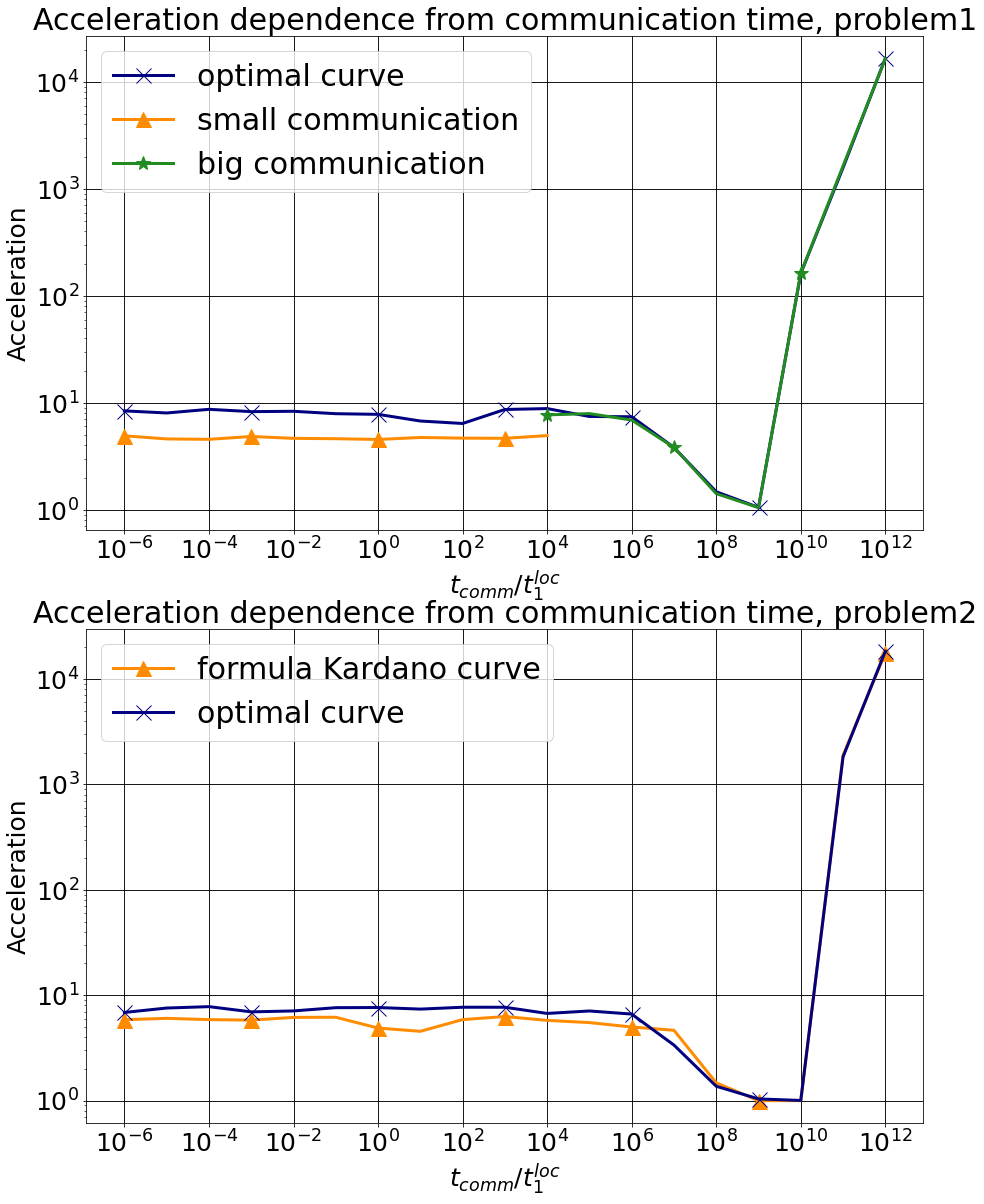
\includegraphics[width=1\linewidth]{графики.png}}
\caption{}
\label{ris:image}
\end{figure}

Проанализируем полученные графики. Формула для случая больших коммуникаций и формула Кардано практически совпали с оптимальным поиском решения. Случай малых коммуникаций показал результаты хуже. Это объясняется тем, что формула была получена в грубом приближении. Но, если учесть константы $\alpha, \beta$, то можно получить лучший результат, что показано далее.






\bibliographystyle{unsrtnat}
\bibliography{refs}  


\end{document}